\documentclass[a4paper, 14pt]{extarticle}

% Поля
%--------------------------------------
\usepackage{geometry}
\geometry{a4paper,tmargin=2cm,bmargin=2cm,lmargin=3cm,rmargin=1cm}
%--------------------------------------


%Russian-specific packages
%--------------------------------------
\usepackage[T2A]{fontenc}
\usepackage[utf8]{inputenc} 
\usepackage[english, main=russian]{babel}
%--------------------------------------

\usepackage{textcomp}

% Красная строка
%--------------------------------------
\usepackage{indentfirst}               
%--------------------------------------             


%Graphics
%--------------------------------------
\usepackage{graphicx}
\graphicspath{ {./images/} }
\usepackage{wrapfig}
%--------------------------------------

% Полуторный интервал
%--------------------------------------
\linespread{1.3}                    
%--------------------------------------

%Выравнивание и переносы
%--------------------------------------
% Избавляемся от переполнений
\sloppy
% Запрещаем разрыв страницы после первой строки абзаца
\clubpenalty=10000
% Запрещаем разрыв страницы после последней строки абзаца
\widowpenalty=10000
%--------------------------------------

%Списки
\usepackage{enumitem}

%Подписи
\usepackage{caption} 

%Гиперссылки
\usepackage{hyperref}

\hypersetup {
	unicode=true
}

%Рисунки
%--------------------------------------
\DeclareCaptionLabelSeparator*{emdash}{~--- }
\captionsetup[figure]{labelsep=emdash,font=onehalfspacing,position=bottom}
%--------------------------------------

\usepackage{tempora}

%Листинги
%--------------------------------------
\usepackage{listings}
\lstset{
  basicstyle=\ttfamily\footnotesize, 
  %basicstyle=\footnotesize\AnkaCoder,        % the size of the fonts that are used for the code
  breakatwhitespace=false,         % sets if automatic breaks shoulbd only happen at whitespace
  breaklines=true,                 % sets automatic line breaking
  captionpos=t,                    % sets the caption-position to bottom
  inputencoding=utf8,
  frame=single,                    % adds a frame around the code
  keepspaces=true,                 % keeps spaces in text, useful for keeping indentation of code (possibly needs columns=flexible)
  keywordstyle=\bf,       % keyword style
  numbers=left,                    % where to put the line-numbers; possible values are (none, left, right)
  numbersep=5pt,                   % how far the line-numbers are from the code
  xleftmargin=25pt,
  xrightmargin=25pt,
  showspaces=false,                % show spaces everywhere adding particular underscores; it overrides 'showstringspaces'
  showstringspaces=false,          % underline spaces within strings only
  showtabs=false,                  % show tabs within strings adding particular underscores
  stepnumber=1,                    % the step between two line-numbers. If it's 1, each line will be numbered
  tabsize=2,                       % sets default tabsize to 8 spaces
  title=\lstname                   % show the filename of files included with \lstinputlisting; also try caption instead of title
}
%--------------------------------------

%%% Математические пакеты %%%
%--------------------------------------
\usepackage{amsthm,amsfonts,amsmath,amssymb,amscd}  % Математические дополнения от AMS
\usepackage{mathtools}                              % Добавляет окружение multlined
\usepackage[perpage]{footmisc}
%--------------------------------------

%--------------------------------------
%			НАЧАЛО ДОКУМЕНТА
%--------------------------------------

\begin{document}

%--------------------------------------
%			ТИТУЛЬНЫЙ ЛИСТ
%--------------------------------------
\begin{titlepage}
\thispagestyle{empty}
\newpage


%Шапка титульного листа
%--------------------------------------
\vspace*{-60pt}
\hspace{-65pt}
\begin{minipage}{0.3\textwidth}
\hspace*{-20pt}\centering

\includegraphics[width=\textwidth]{emblem}
\end{minipage}
\begin{minipage}{0.67\textwidth}\small \textbf{
\vspace*{-0.7ex}
\hspace*{-6pt}\centerline{Министерство науки и высшего образования Российской Федерации}
\vspace*{-0.7ex}
\centerline{Федеральное государственное бюджетное образовательное учреждение }
\vspace*{-0.7ex}
\centerline{высшего образования}
\vspace*{-0.7ex}
\centerline{<<Московский государственный технический университет}
\vspace*{-0.7ex}
\centerline{имени Н.Э. Баумана}
\vspace*{-0.7ex}
\centerline{(национальный исследовательский университет)>>}
\vspace*{-0.7ex}
\centerline{(МГТУ им. Н.Э. Баумана)}}
\end{minipage}
%--------------------------------------

%Полосы
%--------------------------------------
\vspace{-25pt}
\hspace{-35pt}\rule{\textwidth}{2.3pt}

\vspace*{-20.3pt}
\hspace{-35pt}\rule{\textwidth}{0.4pt}
%--------------------------------------

\vspace{1.5ex}
\hspace{-35pt} \noindent \small ФАКУЛЬТЕТ\hspace{80pt} <<Информатика и системы управления>>

\vspace*{-16pt}
\hspace{47pt}\rule{0.83\textwidth}{0.4pt}

\vspace{0.5ex}
\hspace{-35pt} \noindent \small КАФЕДРА\hspace{50pt} <<Теоретическая информатика и компьютерные технологии>>

\vspace*{-16pt}
\hspace{30pt}\rule{0.866\textwidth}{0.4pt}
  
\vspace{11em}

\begin{center}
\Large {\bf Лабораторная работа № 5} \\ 
\large {\bf по курсу <<Компьютерные сети>>} \\
\large <<Реализация WebSocket клиента и сервера
на языке Golang>> 
\end{center}\normalsize

\vspace{8em}


\begin{flushright}
  {Студент группы ИУ9-32Б Волохов А. В. \hspace*{15pt}\\ 
  \vspace{2ex}
  Преподаватель Посевин Д. П.\hspace*{15pt}}
\end{flushright}

\bigskip

\vfill
 

\begin{center}
\textsl{Москва 2023}
\end{center}
\end{titlepage}
%--------------------------------------
%		КОНЕЦ ТИТУЛЬНОГО ЛИСТА
%--------------------------------------

\renewcommand{\ttdefault}{pcr}

\setlength{\tabcolsep}{3pt}
\newpage
\setcounter{page}{2}
\section{Задание}\label{Sect::task}

Исходный код программы представлен в листингах~\ref{lst:code1}--~\ref{lst:code2}--~\ref{lst:code3}--~\ref{lst:code4}--~\ref{lst:code5}--~\ref{lst:code6}.

\begin{figure}[!htb]
\begin{lstlisting}[language={Go},caption={client.go},label={lst:code1}]
package main
import (
	"bufio"
	"fmt"
	"github.com/gorilla/websocket"
	"os"
	"strconv"
)
type Process struct {
	PID         int    `json:"pid"`
	ProcessName string `json:"processName,omitempty"`
	Error       string `json:"error,omitempty"`
}
func main() {
	conn, _, err := websocket.DefaultDialer.Dial("ws://localhost:8080", nil)
	if err != nil {
		fmt.Println(err)
		return
	}
	defer func(conn *websocket.Conn) {
		err := conn.Close()
		if err != nil {

		}
	}(conn)
	for {
		fmt.Print("Enter PID: ")
		scanner := bufio.NewScanner(os.Stdin)
		scanner.Scan()
		pidStr := scanner.Text()
		pid, err := strconv.Atoi(pidStr)
		if err != nil {
			fmt.Println("Error: Invalid PID. Please enter a valid number.")
			continue
		}
		processData := Process{
			PID: pid,
		}
		err = conn.WriteJSON(processData)
		if err != nil {
			fmt.Println(err)
			break
		}
		var responseData Process
		err = conn.ReadJSON(&responseData)
		if err != nil {
			fmt.Println(err)
			break
		}
		if responseData.Error != "" {
			fmt.Printf("Error: %s\n", responseData.Error)
		} else {
			fmt.Printf("Process Name: %s", responseData.ProcessName)
		}
	}
}

\end{lstlisting}
\end{figure}

\newpage

\begin{figure}[!htb]
\begin{lstlisting}[language={Go},caption={server.go},label={lst:code2}]
package main

import (
	"fmt"
	"github.com/gorilla/websocket"
	"io/ioutil"
	"net/http"
	"path/filepath"
	"runtime"
	"strconv"
)

var upgrader = websocket.Upgrader{
	CheckOrigin: func(r *http.Request) bool {
		return true
	},
}

type Process struct {
	PID         int    `json:"pid"`
	ProcessName string `json:"processName,omitempty"`
	Error       string `json:"error,omitempty"`
}

func getProcessName(pid int) (string, error) {
	var processName string

	switch runtime.GOOS {
	case "linux", "darwin":
		commPath := filepath.Join("/proc", strconv.Itoa(pid), "comm")
		data, err := ioutil.ReadFile(commPath)
		if err != nil {
			return "", err
		}
		processName = string(data)
	default:
		return "", fmt.Errorf("unsupported operating system")
	}

	return processName, nil
}

func handleConnection(w http.ResponseWriter, r *http.Request) {
	conn, err := upgrader.Upgrade(w, r, nil)
	if err != nil {
		fmt.Println(err)
		return
	}
	defer func(conn *websocket.Conn) {
		err := conn.Close()
		if err != nil {

		}
	}(conn)

\end{lstlisting}
\end{figure}

\newpage
\begin{figure}[!htb]
\begin{lstlisting}[language={Go},caption={server.go - продолжение},label={lst:code3}]
for {
		var process Process

		// Чтение входных данных от клиента
		err := conn.ReadJSON(&process)
		if err != nil {
			fmt.Println(err)
			break
		}

		processName, err := getProcessName(process.PID)
		if err != nil {
			// Если произошла ошибка, добавляем ее в OutputData
			process.Error = err.Error()
		} else {
			// Если ошибки нет, добавляем имя процесса
			process.ProcessName = processName
		}

		// Отправка данных обратно клиенту
		err = conn.WriteJSON(process)
		if err != nil {
			fmt.Println(err)
			break
		}
	}
}

func main() {
	http.HandleFunc("/", handleConnection)
	fmt.Println("Server is listening on :8080")
	err := http.ListenAndServe(":8080", nil)
	if err != nil {
		return
	}
}
	
\end{lstlisting}
\end{figure}

\newpage

\begin{figure}[!htb]
	\centering
	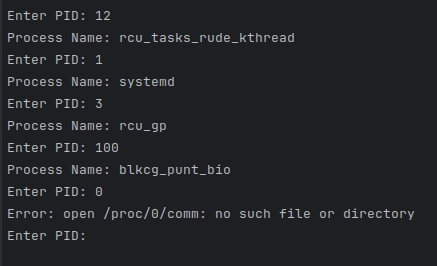
\includegraphics[width=0.8\textwidth]{res.png}
\caption{Пример работы}
\label{fig:img1}
\end{figure}





\end{document}
